\documentclass[11pt, a4paper]{article}
%\usepackage{proj1}
\usepackage{natbib}
\usepackage{fancyhdr}  
\usepackage{subcaption}
\usepackage{caption}
\usepackage{graphicx}
\usepackage{numprint}
\usepackage{multirow}
\linespread{1.25} 
\setlength{\parindent}{0cm}
\graphicspath{{Images/}}
\usepackage{hyperref}
\usepackage{amsmath}
\usepackage{amsfonts}
\usepackage{amssymb}
\usepackage{amsthm}
\usepackage{mathtools}
\usepackage{commath}
\usepackage{bbm}

%\usepackage[sc,osf]{mathpazo}
\usepackage{subcaption}
\usepackage[a4paper, top=1in, left=1.0in, right=1.0in, bottom=1in, includehead, includefoot]{geometry} %Usually have top as 1in

\usepackage{listings}
\usepackage{color} %red, green, blue, yellow, cyan, magenta, black, white
\definecolor{mygreen}{RGB}{28,172,0} % color values Red, Green, Blue
\definecolor{mylilas}{RGB}{170,55,241}


\hypersetup{colorlinks,linkcolor={black},citecolor={blue},urlcolor={black}}
\usepackage{color}
\urlstyle{same}


\theoremstyle{definition}
\newtheorem{definition}{Definition}[section]

\newcommand{\adja}{q_a}
\newcommand{\adjb}{q_b}
\newcommand{\adjaB}{q_{a,\partial \Omega}}
\newcommand{\adjbB}{q_{b,\partial \Omega}}
\newcommand{\adjB}{q_{\partial \Omega}}
\newcommand{\Adja}{\mathbf{p}}
\newcommand{\Adjb}{q}
\newcommand{\adj}{q}
\newcommand{\Adjc}{{q}_{\partial \Omega}}
\newcommand{\ra}{\rho_a}
\newcommand{\rb}{\rho_b}
\newcommand{\w}{\mathbf{w}}
\newcommand{\f}{\mathbf{f}}
\newcommand{\ve}{\mathbf{v}}
\newcommand{\n}{\mathbf{n}}
\newcommand{\h}{\mathbf{h}}
\newcommand{\K}{\mathbf{K}}
\newcommand{\hr}{\widehat \rho}

%	\begin{figure}[h]
%		\centering
%		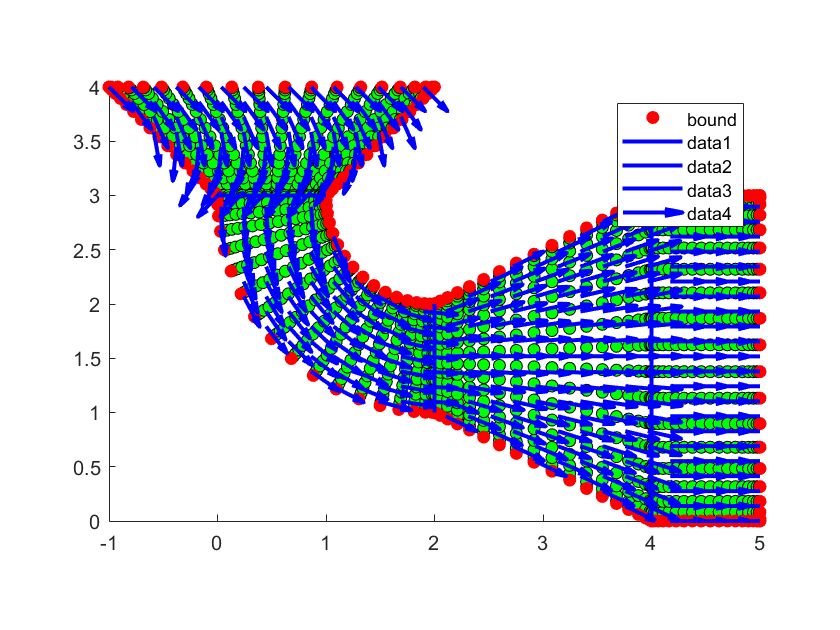
\includegraphics[scale=0.35]{F1.png}
%		\caption{Forward $\rho$ for $a = 0.01$} 
%		\label{F1}
%	\end{figure}

\begin{document}
	
	
\section{Averaging the advection-diffusion equation}
We consider the standard advection-diffusion optimality system, with flow control and Neumann boundary conditions:
\begin{align*}
	\frac{\partial \rho}{\partial t} &= \nabla^2 \rho - \nabla \cdot (\rho \w) + f\\
	0 &= (- \nabla \rho + \rho \w) \cdot \n \\
	\\
	\frac{\partial q}{\partial t} &= - \nabla^2 q - \w \cdot \nabla q - \rho + \hr\\
	0 &= \nabla q \cdot \n \\
	\\
	\w &= - \frac{1}{\beta}\rho \nabla q
\end{align*}
We now have the following operators in polar coordinates acting on a function $f$ and a vector field $\w$:
\begin{align*}
	\nabla^2 f &= \frac{1}{r} \frac{\partial}{\partial r} \left( r \frac{\partial f}{\partial r}\right) + \frac{1}{r^2} \frac{\partial^2 f}{\partial \theta^2} + \frac{\partial f}{\partial z^2}\\
	\nabla f &= \left(\frac{\partial f}{\partial r}, \frac{1}{r}\frac{\partial f}{\partial \theta}, \frac{\partial f}{\partial z}\right)\\
	\nabla \cdot \w &= \frac{1}{r}\frac{\partial }{\partial r}\left(r \w_r\right) - \frac{1}{r}\frac{\partial \w_\theta}{\partial \theta} + \frac{\partial \w_z}{\partial z}
\end{align*}
Implementing these, we get:
\begin{align*}
	\frac{\partial \rho}{\partial t} &= \frac{1}{r} \frac{\partial}{\partial r} \left( r \frac{\partial \rho}{\partial r}\right) + \frac{1}{r^2} \frac{\partial^2 \rho}{\partial \theta^2} + \frac{\partial \rho}{\partial z^2} - \frac{1}{r}\frac{\partial }{\partial r}\left(r \rho\w_r\right) + \frac{1}{r}\frac{\partial \rho\w_\theta}{\partial \theta} - \frac{\partial \rho\w_z}{\partial z} + f\\
	0 &= \left(- \left(\frac{\partial \rho}{\partial r}, \frac{1}{r}\frac{\partial \rho}{\partial \theta}, \frac{\partial \rho}{\partial z}\right) + \rho \w \right) \cdot \n \\
	\\
	\frac{\partial q}{\partial t} &= -  \frac{1}{r} \frac{\partial}{\partial r} \left( r \frac{\partial q}{\partial r}\right) - \frac{1}{r^2} \frac{\partial^2 fq}{\partial \theta^2} - \frac{\partial q}{\partial z^2} - \w \cdot \left(\frac{\partial q}{\partial r}, \frac{1}{r}\frac{\partial q}{\partial \theta}, \frac{\partial q}{\partial z}\right) - \rho + \hr\\
	0 &= \left(\frac{\partial q}{\partial r}, \frac{1}{r}\frac{\partial q}{\partial \theta}, \frac{\partial q}{\partial z}\right) \cdot \n \\
	\\
	\w &= - \frac{1}{\beta}\rho  \left(\frac{\partial q}{\partial r}, \frac{1}{r}\frac{\partial q}{\partial \theta}, \frac{\partial q}{\partial z}\right)
\end{align*}
Then we set $\theta$ to be constant, so that all derivatives in $\theta$ are zero and we multiply out some derivatives, to get:

\begin{align*}
	\frac{\partial \rho}{\partial t} &= \frac{1}{r} \frac{\partial \rho}{\partial r} +  \frac{\partial^2 \rho}{\partial r^2} + \frac{\partial \rho}{\partial z^2} - \frac{\rho\w_r}{r} -\rho\frac{\partial \w_r }{\partial r} -\w_r\frac{\partial \rho}{\partial r} - \rho\frac{\partial \w_z}{\partial z}- \w_z\frac{\partial \rho}{\partial z} + f\\
	0 &= \left(- \left(\frac{\partial \rho}{\partial r},  \frac{\partial \rho}{\partial z}\right) + \rho \w \right) \cdot \n \\
	\\
	\frac{\partial q}{\partial t} &= - \frac{1}{r} \frac{\partial q}{\partial r} -  \frac{\partial^2 q}{\partial r^2} - \frac{\partial q}{\partial z^2} - \w \cdot \left(\frac{\partial q}{\partial r},  \frac{\partial q}{\partial z}\right) - \rho + \hr\\
	0 &= \left(\frac{\partial q}{\partial r},  \frac{\partial q}{\partial z}\right) \cdot \n \\
	\\
	\w &= - \frac{1}{\beta}\rho  \left(\frac{\partial q}{\partial r},  \frac{\partial q}{\partial z}\right)
\end{align*}
We can rewrite some of the terms in the forward equation:
\begin{align*}
	-\w_r\frac{\partial \rho}{\partial r} - \w_z\frac{\partial \rho}{\partial z} &= - \left(\w \cdot \nabla \right)\rho\\
	-\rho\frac{\partial \w_r }{\partial r} - \rho\frac{\partial \w_z}{\partial z} &= -\left(\nabla \cdot \w \right)\rho 
\end{align*}
Using the vector identity $\mathbf a (\nabla \cdot \mathbf b) + (\mathbf b \cdot \nabla ) \mathbf a = \nabla \cdot (\mathbf{b a^T})$, we get that the above two terms become:
\begin{align*}
	- \left(\w \cdot \nabla \right)\rho - \left(\nabla \cdot \w \right)\rho = - \nabla \cdot (\rho\w ).
\end{align*}

Then the optimality system is:
\begin{align*}
	\frac{\partial \rho}{\partial t} &= \frac{1}{r} \frac{\partial \rho}{\partial r} +  \frac{\partial^2 \rho}{\partial r^2} + \frac{\partial \rho}{\partial z^2} - \frac{\rho\w_r}{r} - \nabla \cdot (\rho \w ) + f\\
	0 &= \left(- \left(\frac{\partial \rho}{\partial r},  \frac{\partial \rho}{\partial z}\right) + \rho \w \right) \cdot \n \\
	\\
	\frac{\partial q}{\partial t} &= - \frac{1}{r} \frac{\partial q}{\partial r} -  \frac{\partial^2 q}{\partial r^2} - \frac{\partial q}{\partial z^2} - \w \cdot \left(\frac{\partial q}{\partial r},  \frac{\partial q}{\partial z}\right) - \rho + \hr\\
	0 &= \left(\frac{\partial q}{\partial r},  \frac{\partial q}{\partial z}\right) \cdot \n \\
	\\
	\w &= - \frac{1}{\beta}\rho  \left(\frac{\partial q}{\partial r},  \frac{\partial q}{\partial z}\right)
\end{align*}

\subsection{Exact Solution}
We are choosing an exact solution which satisfies the boundary conditions, matches the final time condition for $q$ and is invariant in $\theta$. We choose:
\begin{align*}
	\rho &= \beta^{1/2} e^t \cos(\pi r) \cos (\pi z)\\
	q &= \beta^{1/2}(e^T - e^t)\cos(\pi r)\cos(\pi z),
\end{align*}
and use these to determine the values of $\w$, $f$ and $\hr$.
\\
\\
There must be a mistake somewhere because the exact solution is still not exact. I am not sure what this mistake is yet.

	
\end{document}